\chapter{Martensitbildung}
\label{MB1}

\section{Durchführung (ZB)}

In diesem Schritt soll das bimodale Gefüge durch Bildung von feinen Martensit-Nadeln verfeinert und dadurch verfestigt werden. Um das zu erreichen, werden Ti-64-Proben nach \cite{Morita.2005} nach dem Duplex Anneal 3 Minuten bei 930 geglüht und dann Wasserabgeschrekt. Bei der Erwährmung sollen die Beta Lamellen im transformierten Beta Wachsen, indem sich ein Anteil der Alpha-lamellen in Beta umwandelt (Siehe Abbildung \ref{fig:martensit-einzeln} ).

\begin{figure}
	\centering
	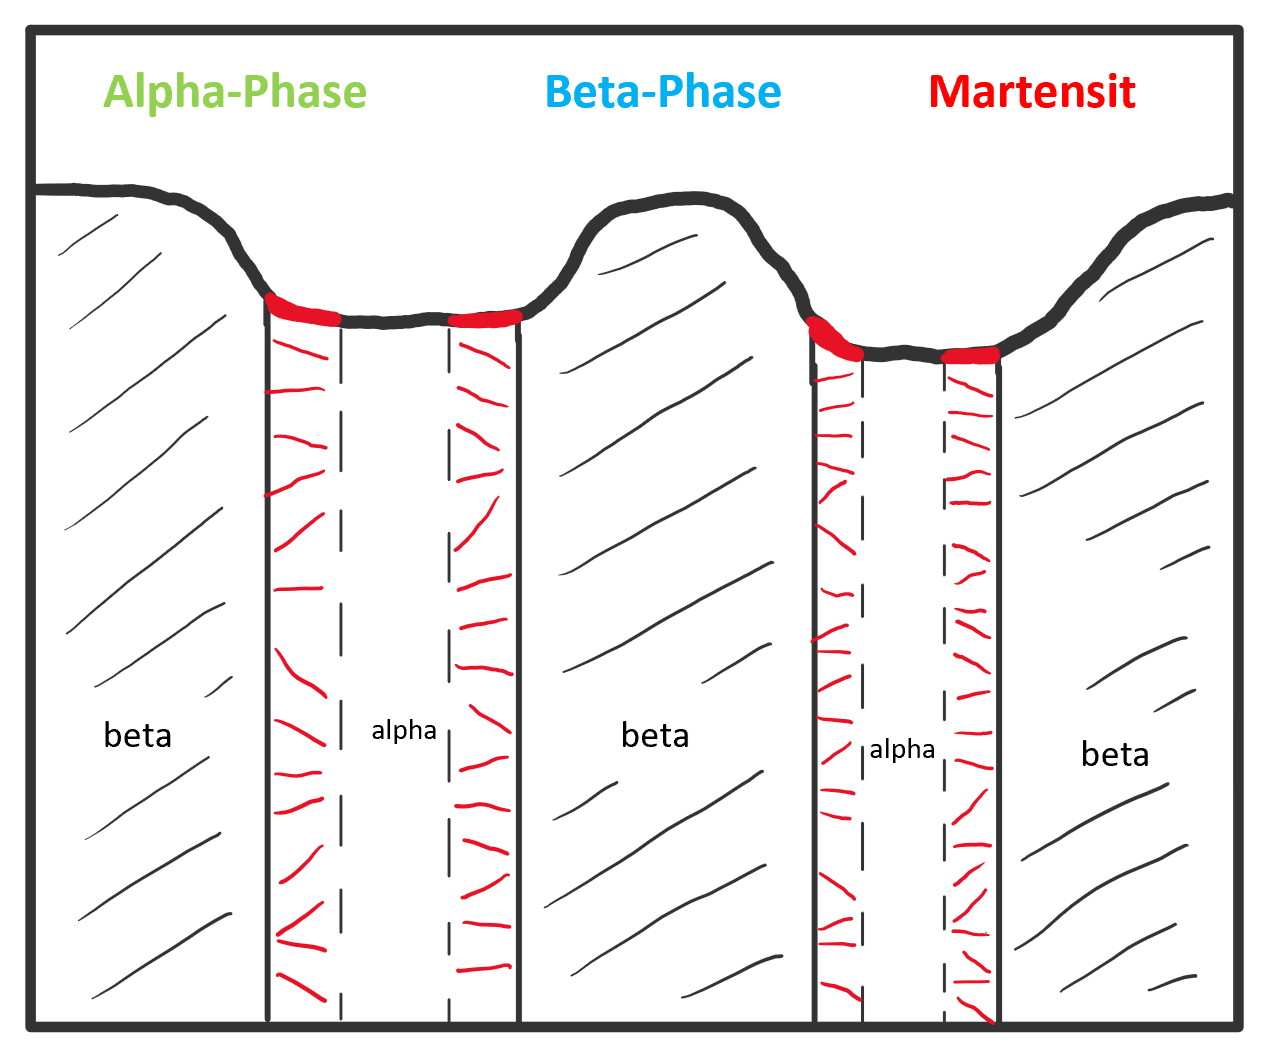
\includegraphics[width=0.7\linewidth]{./Bilder/Martensit einzeln.png}
	\caption{Wachstum der $\beta$-Lamellen bei erhöhung der Temperatur eines Duplex-Gefüges}
	\label{fig:martensit-einzeln}
\end{figure}

Innerhalb der kurzen Anlasszeit können die $\beta$-Stabilisatoren, bei Ti-64 Vanadium, in den neu-gebildeten $\beta$-Gebieten nicht diffundieren. Deshalb wandeln sich diese instabilen $\beta$-Gebiete beim Abschrecken diffusionslos in Martensit um.\\

Die T$_\beta$ von Ti-6242 ist aufgrund des niedrigen Mo-Gehalts höher als die von Ti-64.Das bedeutet, dass die Umwandlungsvorgänge $\alpha$ --> $\beta$ von Ti-6242 langsamer sind als die von Ti-64 bei der selben Temperatur. Deshalb wurden in diesem Schritt Ti-6242-Proben bei 930$^\circ$C und 950$^\circ$C  geglüht. Außerdem sind die im Rahmen dieses Projekts verwendeten Proben dicker als die im \cite{Morita.2005} genommenen Ti-64-Proben und wurden daher für 8 und 16 min angelassen.

\section{Ergebnisse (PH)}

Im nächsten Schritt wurde versucht, die STDA-Wärmebehandlung von der $\alpha$+$\beta$-Legierung Ti-6Al-4V auf die near-$\alpha$-Legierung Ti-6Al-2Sn-4Zr-2Mo zu übertragen. Ziel war es zunächst in einem zweiten Prozessschritt Martensit in der $\beta$-Phase zu erzeugen. Dafür wurden die Proben mit bi-modalen Mikrostrukturen aus der ersten Wärmebehandlung ($\alpha_p$-Studie) erneut bei 930$^\circ$C im Ofen für 8 Minuten geglüht und anschließend wassergekühlt. Die Auswertung unter dem Lichtmikroskop ist in Abbildung \ref{fig:abbildung-9} zusammengefasst.

\begin{figure}
	\centering
	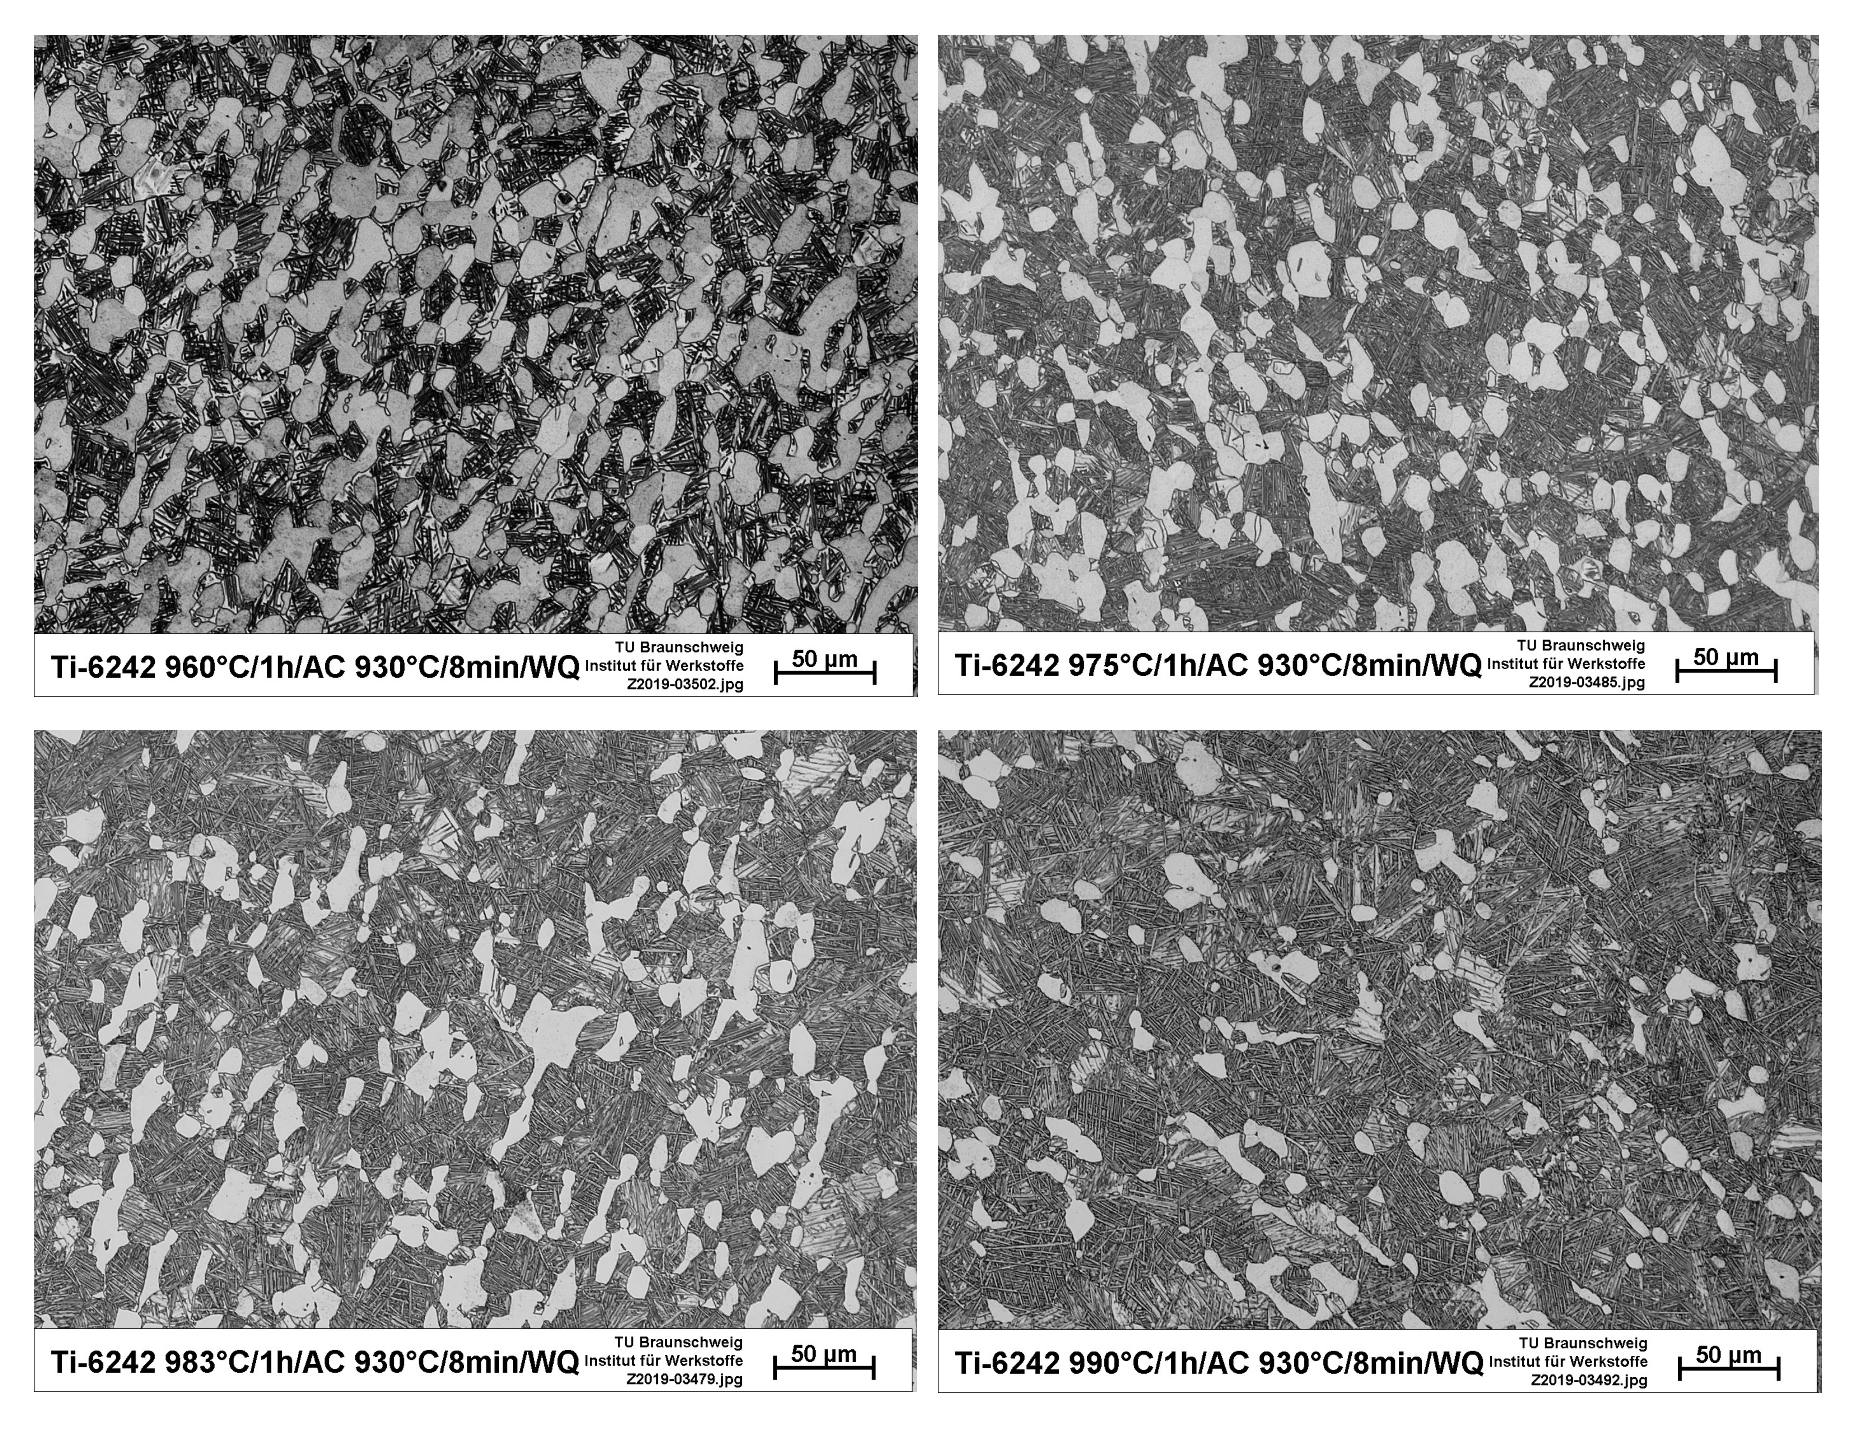
\includegraphics[width=0.9\linewidth]{./Bilder/Abbildung 9.png}
	\caption[Abbildung 9]{Mikrostrukturen von Ti-6242 nach dem zweiten Prozessschritt}
	\label{fig:abbildung-9}
\end{figure}

Nach dem zweiten Prozessschritt konnte keine Veränderung der Mikrostrukturen unter dem Lichtmikroskop zum ersten Schritt festgestellt werden. Daher wurden die Proben unter dem Rasterelektronenmikroskop (REM) näher untersucht, um festzustellen, ob sich Martensit in der $\beta$-Phase geformt hat. Die Ergebnisse sind in Abbildungen \ref{fig:abbildung-10} -- \ref{fig:abbildung-13} aufgeführt. 

Das Martensit in der $\beta$-Phase bildet sich nadelförmig aus. Diese Martensitnadeln entstehen häufig in einem orthogonalem Winkel zueinander. In Abbildung \ref{fig:abbildung-21} sind Beispiele für martensitische Strukturen innerhalb der $\beta$-Phase hervorgehoben.

\begin{figure}
	\centering
	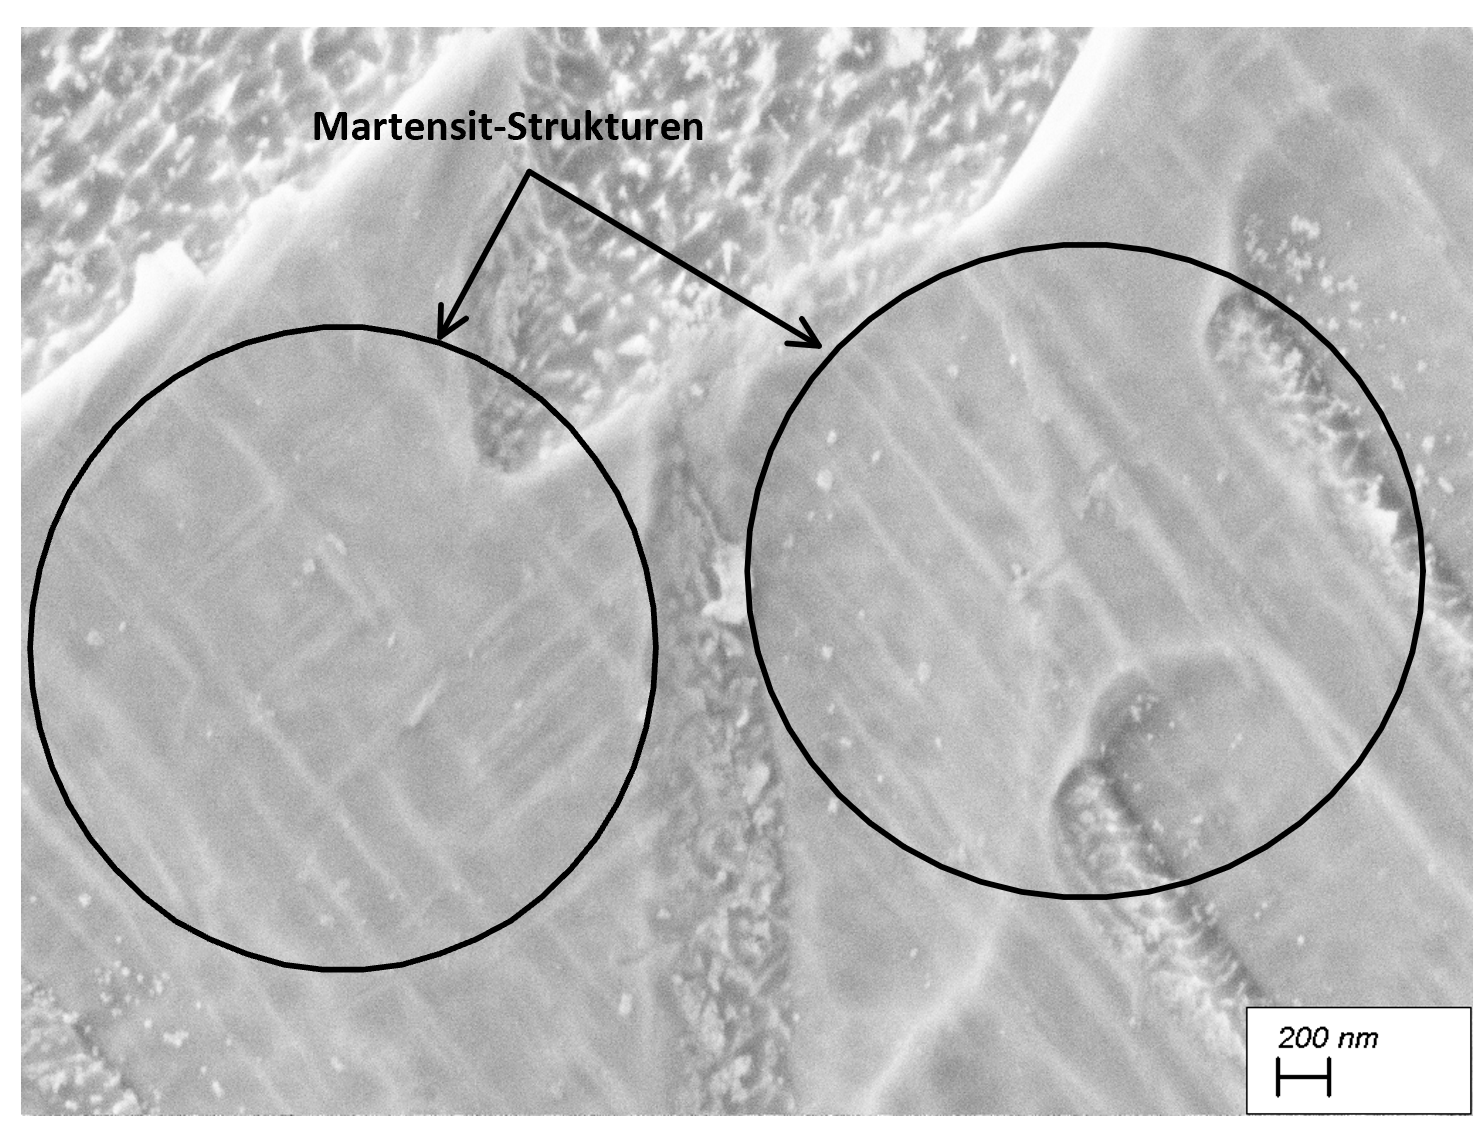
\includegraphics[width=0.8\linewidth]{./Bilder/Abbildung 21.png}
	\caption[Abbildung]{Martensit-Strukturen in der $\beta$-Phase}
	\label{fig:abbildung-21}
\end{figure}

\begin{figure}
	\centering
	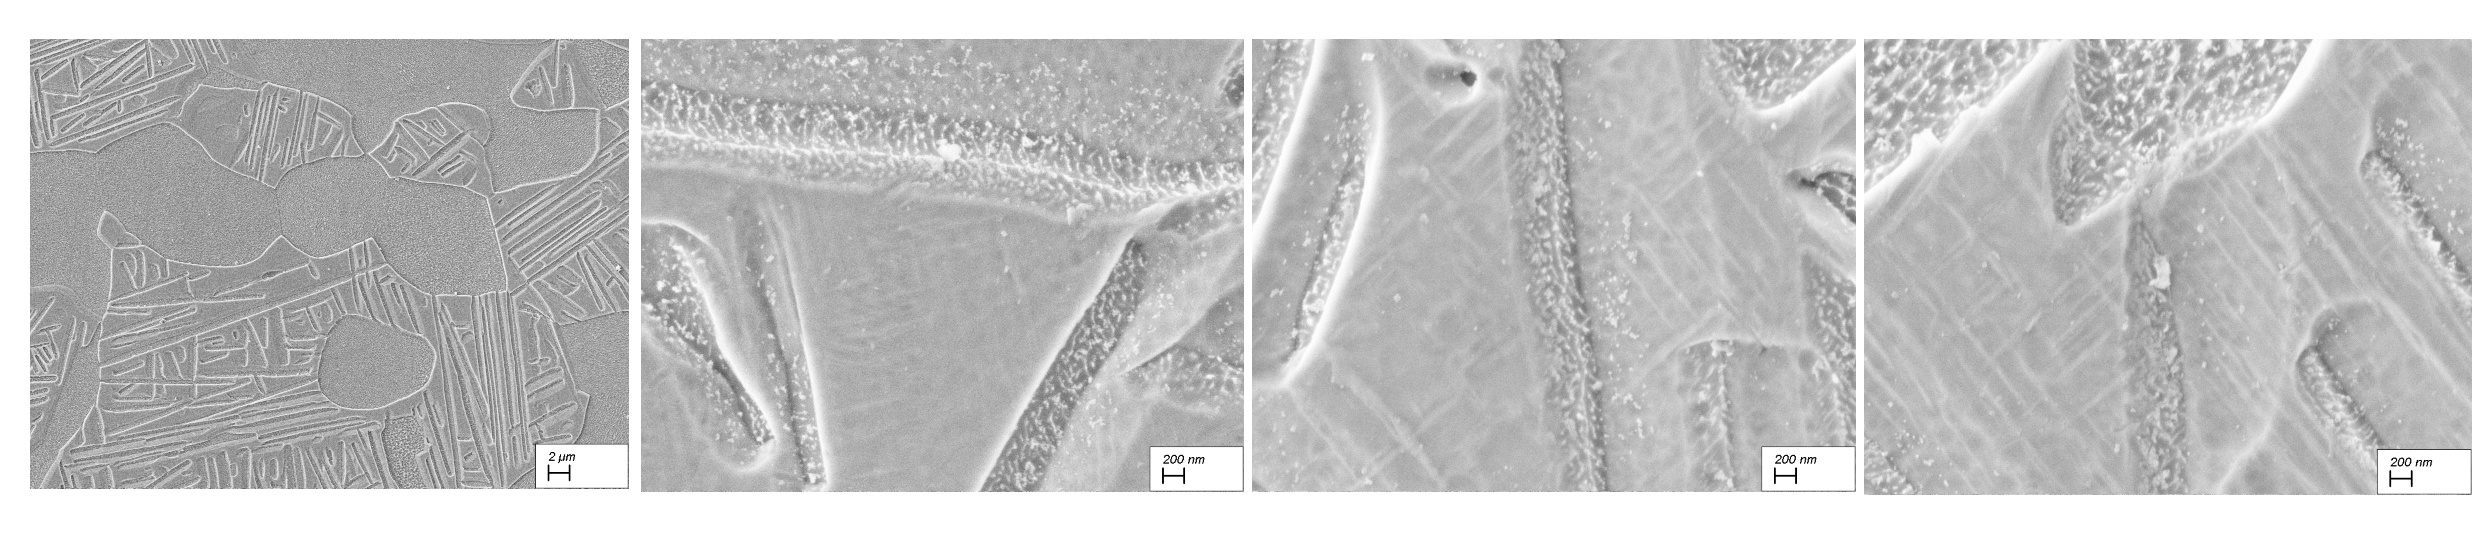
\includegraphics[width=1.0\linewidth]{./Bilder/Abbildung 10.png}
	\caption[Abbildung 10]{960$^\circ$C/1h/AC + 930$^\circ$C/8min/WQ, REM, Randbereich}
	\label{fig:abbildung-10}
\end{figure}

\begin{figure}
	\centering
	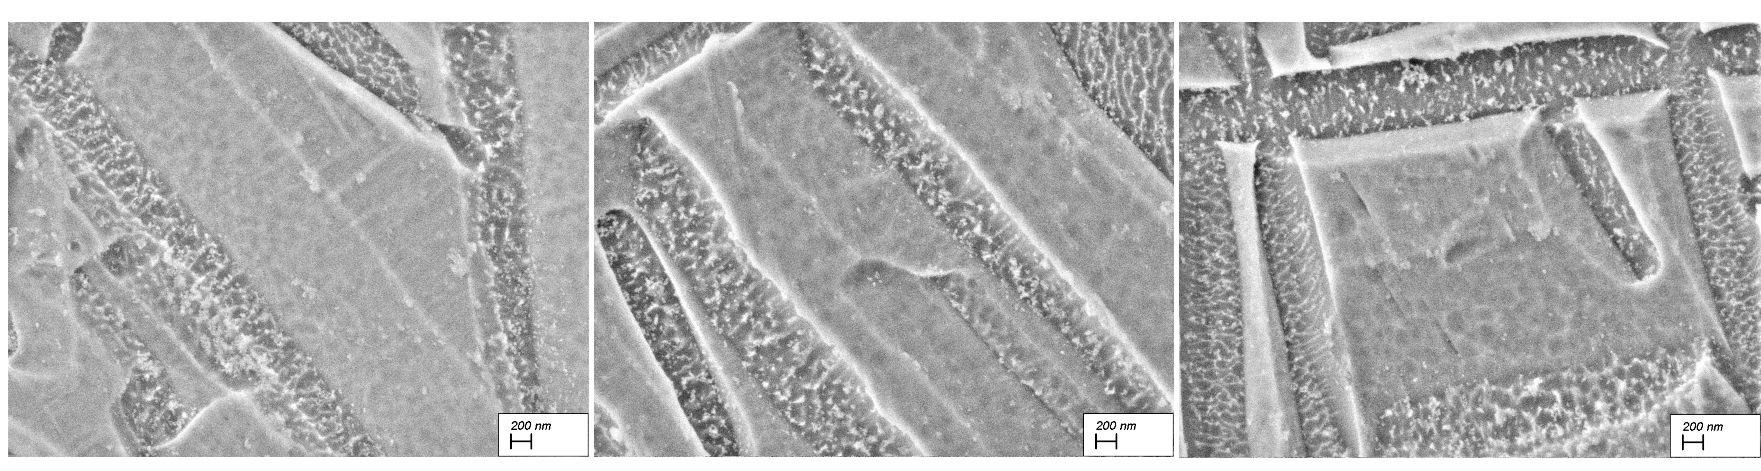
\includegraphics[width=1.0\linewidth]{./Bilder/Abbildung 11.png}
	\caption[Abbildung 11]{975$^\circ$C/1h/AC + 930$^\circ$C/8min/WQ, REM, Randbereich}
	\label{fig:abbildung-11}
\end{figure}

\begin{figure}
	\centering
	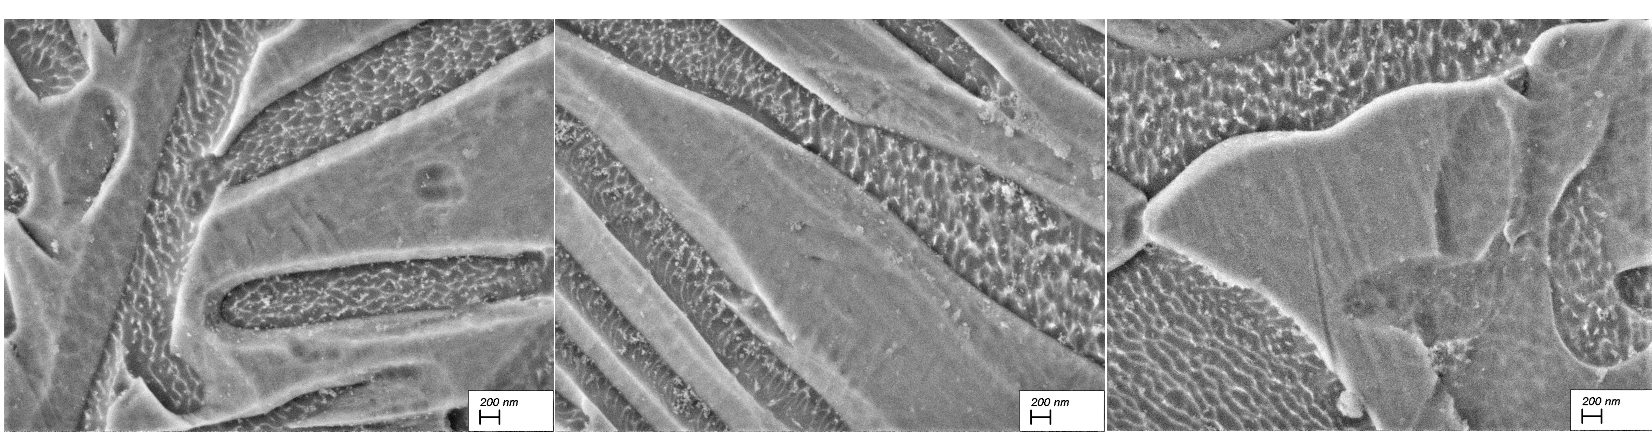
\includegraphics[width=1.0\linewidth]{./Bilder/Abbildung 12.png}
	\caption[Abbildung 12]{983$^\circ$C/1h/AC + 930$^\circ$C/8min/WQ, REM , Randbereich}
	\label{fig:abbildung-12}
\end{figure}

\begin{figure}
	\centering
	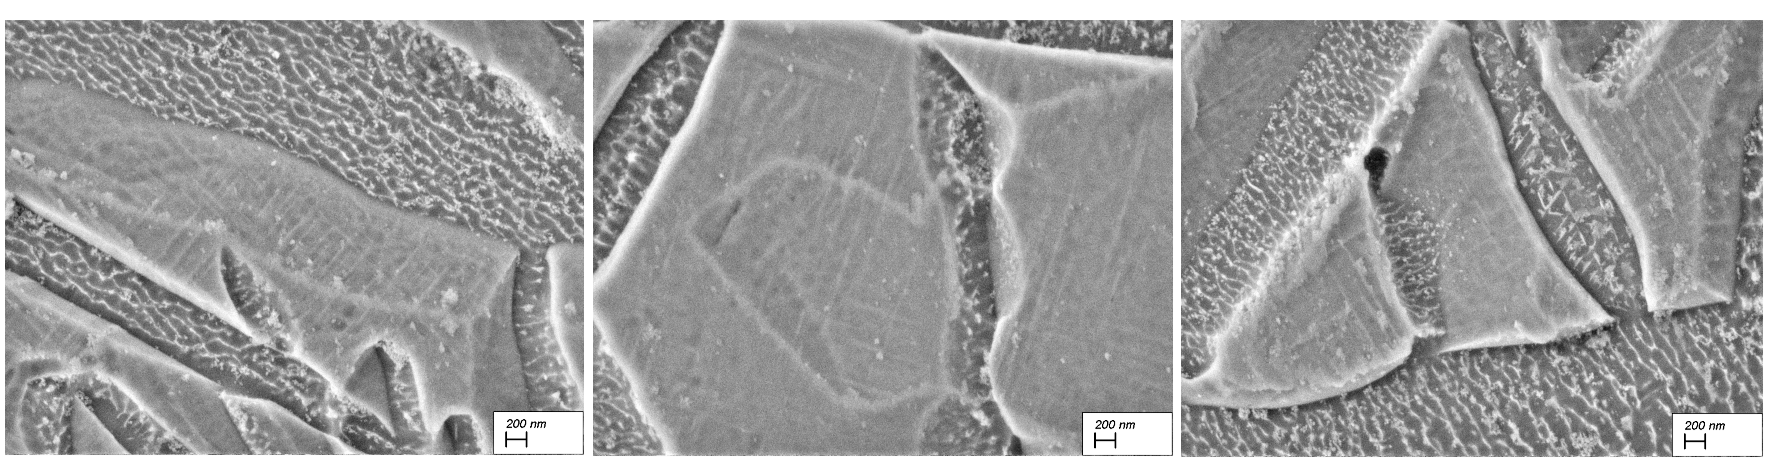
\includegraphics[width=1.0\linewidth]{./Bilder/Abbildung 13.png}
	\caption[Abbildung 13]{990$^\circ$C/1h/AC + 930$^\circ$C/8min/WQ, REM , Randbereich}
	\label{fig:abbildung-13}
\end{figure}

In den Abbildungen \ref{fig:abbildung-10} -- \ref{fig:abbildung-13} ist zu erkennen, dass lediglich die Proben der Temperaturenreihe mit 960$^\circ$C und 990$^\circ$C ansatzweise martensitische Strukturen im Randbereich aufweisen. In den Proben der Temperaturen 975$^\circ$C und 983$^\circ$C sind nur vereinzelt Martensitnadeln zu erkennen. Da diese Temperaturen zwischen 960$^\circ$C und 990$^\circ$C liegen, ist davon auszugehen, dass auch diese Proben stellenweise ausgeprägte Martensitstrukturen aufweisen, jedoch bei der Auswertung unter dem REM nicht gefunden wurden. Die Ergebnisse der folgenden Härteprüfung lässt ebenfalls auf diese Vermutung schließen. Die Qualität der Probenpräparation kann ebenfalls einen Einfluss auf die Sichtbarkeit der Strukturen haben.

Die Härteprüfung dieser Probenreihe ist in Tabelle \ref{Tabelle 6} zusammengefasst, zeigt jedoch bei keiner Probe eine sichtbare Härtesteigerung gegenüber den Werten nach der ersten Wärmebehandlung aus Tabelle \ref{Tabelle 5}.

\begin{table}
	\centering
	\begin{tabular}{|c|c|}
		\hline 
		Probe & Härte in HV \\ 
		\hline 
		960$^\circ$C/1h/AC + 930$^\circ$C/8min/WQ & 350 \\ 
		\hline 
		975$^\circ$C/1h/AC + 930$^\circ$C/8min/WQ & 345 \\ 
		\hline 
		983$^\circ$C/1h/AC + 930$^\circ$C/8min/WQ & 349 \\ 
		\hline 
		990$^\circ$C/1h/AC + 930$^\circ$C/8min/WQ & 352 \\ 
		\hline 
	\end{tabular} 
	\caption{Ergebnisse der Härteprüfung der zweiten Probenreihe}
	\label{Tabelle 6}
\end{table}

Die Ergebnisse dieser Probenreihe entsprach nicht den Erwartungen, da es nur stellenweise zur Martensitbildung im Randbereich kam. Daher wurde dieser zweite Schritt der Wärmebehandlung genauer verfolgt. Ab diesem Punkt wurde im ersten Behandlungsschritt nur noch mit der Temperatur gearbeitet, die in der $\alpha_p$-Studie als Kandidat für den besten $\alpha_p$-Volumenanteil, in Hinblick auf die Zugfestigkeitswerte, ermittelt wurde (983$^\circ$C). 

Um den vorherigen Schritt genauer zu analysieren und optimieren zu können, wurden 3 neue Proben wärmebehandelt. Es wurde daher im zweiten Schritt die Haltezeit der vorherigen Probe verdoppelt. Zusätzlich wurden 2 Proben bei den zwei verschiedenen Haltezeiten (8 und 16 min) mit einer Temperatur geglüht, die um 20$^\circ$C auf 950$^\circ$C angehoben wurde. Dadurch sollten die Einflussfaktoren Temperatur und Haltezeit auf diesen Behandlungsschritt näher untersucht werden, um herauszufinden, warum es nur stellenweise zur Martensitbildung kam. Die Auswertung unter dem Lichtmikroskop ist in Abbildung \ref{fig:abbildung-14} zusammengefasst. 

\begin{figure}
	\centering
	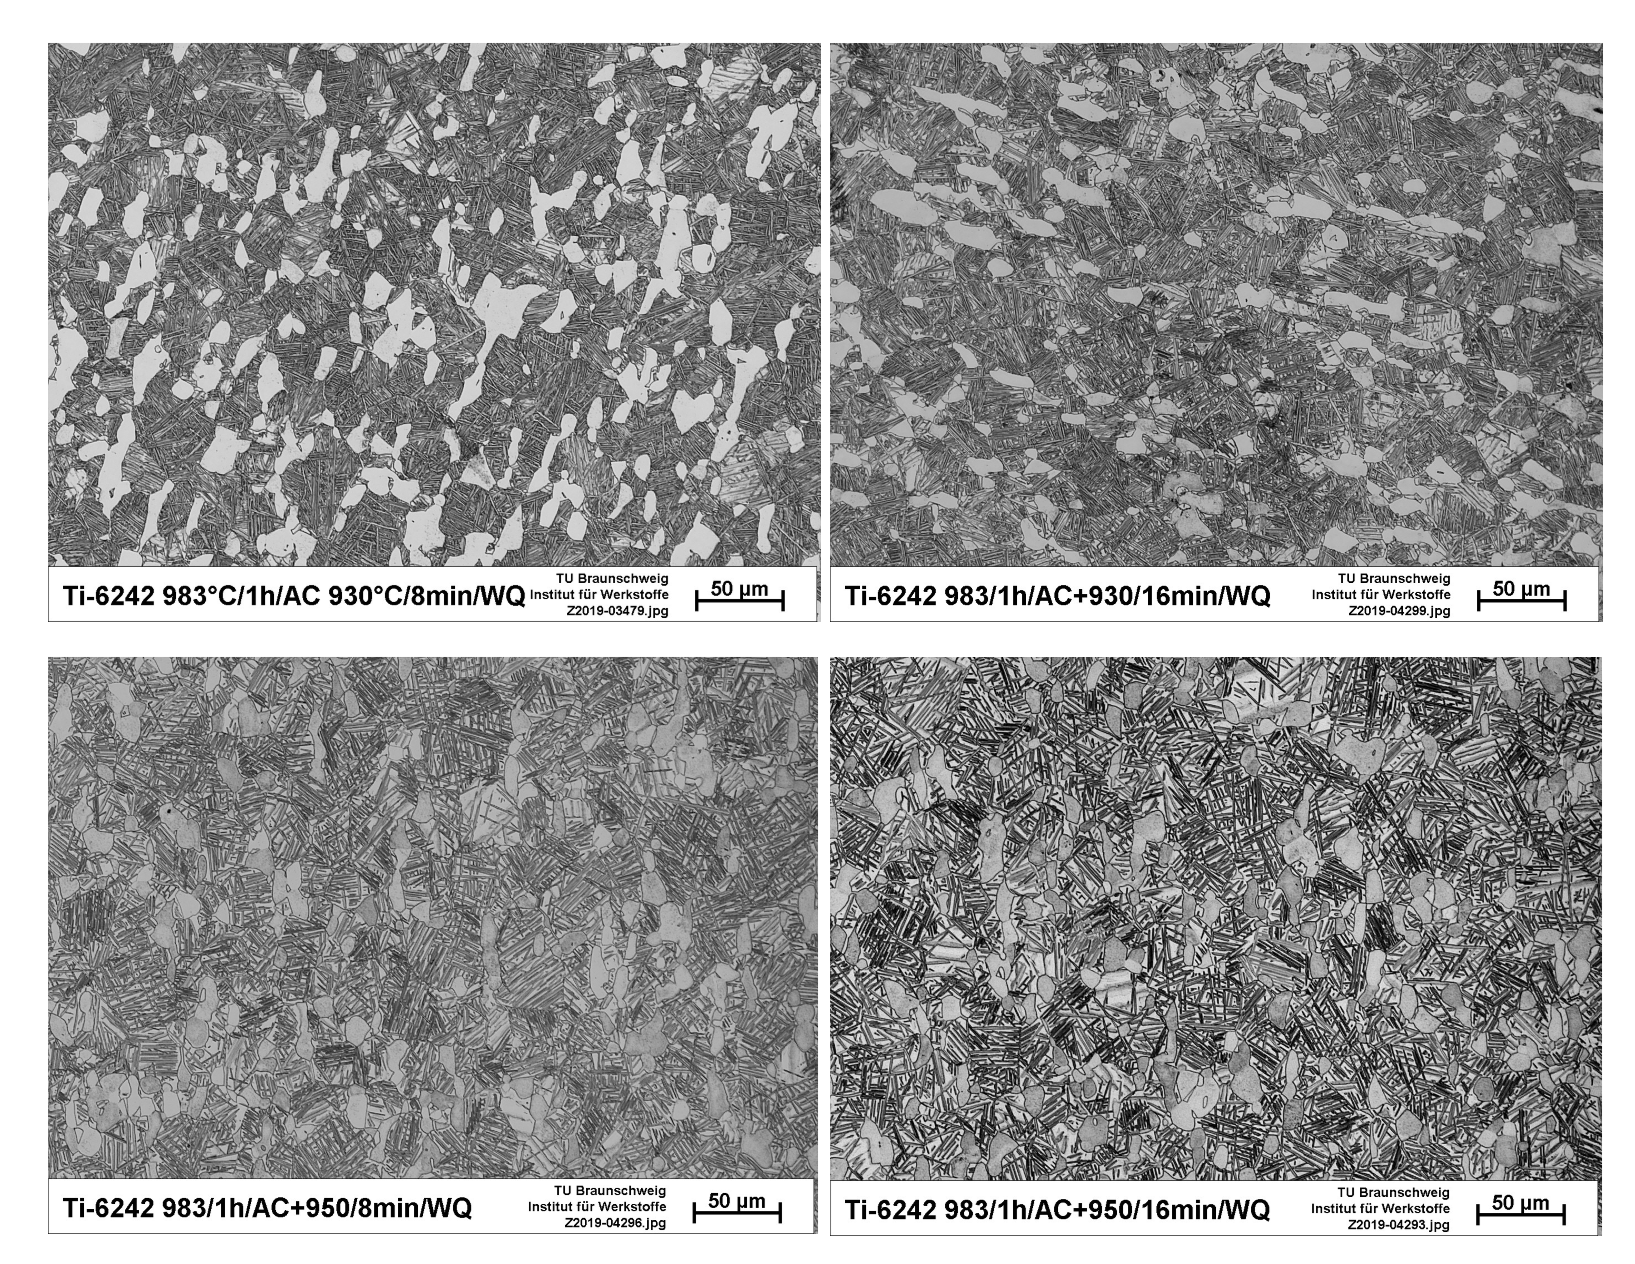
\includegraphics[width=0.9\linewidth]{./Bilder/Abbildung 14.png}
	\caption[Abbildung 14]{Mikrostrukturen nach der Anpassung der Temperatur und Haltezeit im zweiten Wärmebehandlungsschritt}
	\label{fig:abbildung-14}
\end{figure}

Die Proben, die im zweiten Schritt bei 930$^\circ$C geglüht wurden, weisen in ihrer Mikrostruktur keine offensichtlichen Unterschiede zur vorherigen Probenreihe (Abbildung \ref{fig:abbildung-9}) auf. Die Proben, die im zweiten Schritt bei 950$^\circ$C geglüht wurden, weisen eine Veränderung in der $\beta$-Phase auf. So scheint der $\beta$-Phasenanteil zwischen den $\alpha$-Lamellen gewachsen zu sein. Eine Gegenüberstellung der Proben bei 950$^\circ$C und 930$^\circ$C unter dem Lichtmikroskop ist in Abbildung \ref{fig:abbildung-15} zu sehen.

\begin{figure}
	\centering
	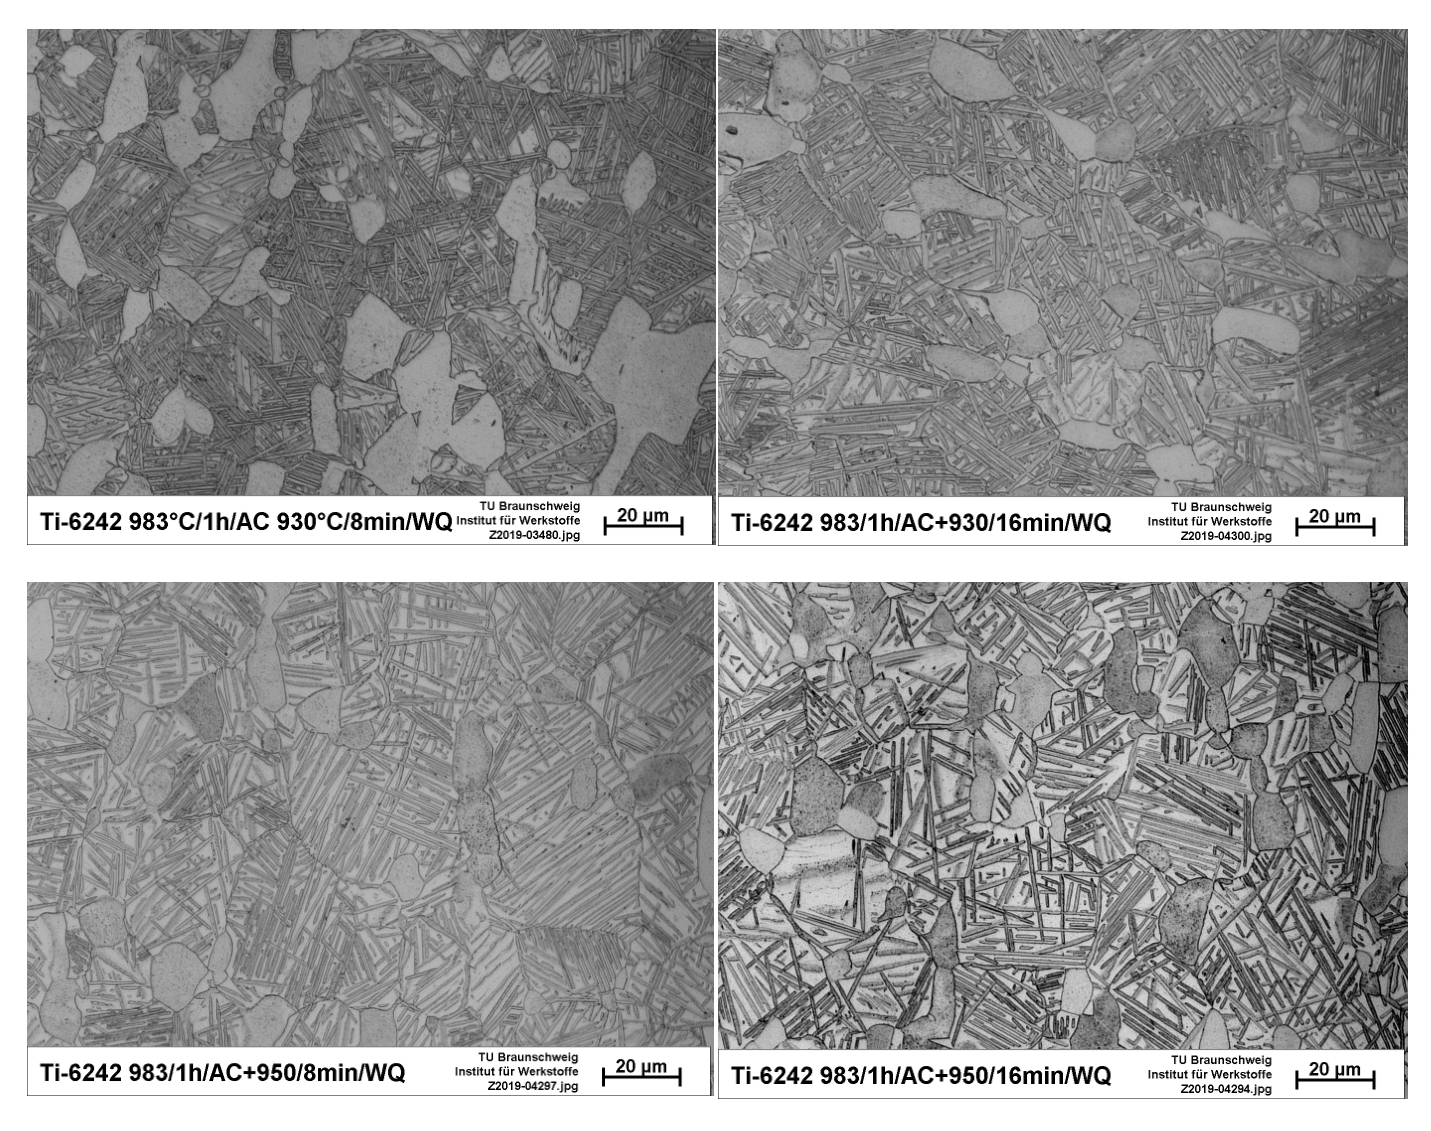
\includegraphics[width=0.9\linewidth]{./Bilder/Abbildung 15.png}
	\caption[Abbildung 15]{Veränderung der $\beta$-Phase im zweiten Wärmebehandlungsschritt bei 950$^\circ$C und 930$^\circ$C}
	\label{fig:abbildung-15}
\end{figure}

Die Härteprüfung der zweiten Probenreihe mit angepassten Temperaturen und Haltezeiten ergab ebenfalls einen Unterschied zur vorherigen Probenreihe. Die Ergebnisse sind in Tabelle \ref{Tabelle 7} aufgeführt.

\begin{table}
	\centering
	\begin{tabular}{|c|c|}
		\hline 
		Probe & Härte in HV \\ 
		\hline 
		983$^\circ$C/1h/AC + 930$^\circ$C/8min/WQ & 349 \\ 
		\hline 
		983$^\circ$C/1h/AC + 930$^\circ$C/16min/WQ & 358 \\ 
		\hline 
		983$^\circ$C/1h/AC + 950$^\circ$C/8min/WQ & 377 \\ 
		\hline 
		983$^\circ$C/1h/AC + 950$^\circ$C/16min/WQ & 376 \\ 
		\hline 
	\end{tabular} 
	\caption{Ergebnisse der Härteprüfung mit angepassten Temperaturen und Haltezeiten}
	\label{Tabelle 7}
\end{table}

Die Härtewerte der Proben, die bei 950$^\circ$C geglüht wurden, weisen eine sichtbare Härtesteigerung gegenüber den Proben, die bei 930$^\circ$C geglüht wurden, auf. Der Wert der Probe, die bei 930$^\circ$C und 16 min geglüht wurde, gegenüber der Probe mit gleicher Temperatur und halber Haltezeit, ist im Rahmen der Genauigkeit nahezu gleich. So zeigt sich, dass in dieser Probenreihe die Haltezeit keinen sichtbaren Einfluss hat. Die nähere Analyse der Mikrostruktur dieser Probenreihe unter dem REM ist in den Abbildungen \ref{fig:abbildung-16} -- \ref{fig:abbildung-18} aufgeführt.

\begin{figure}
	\centering
	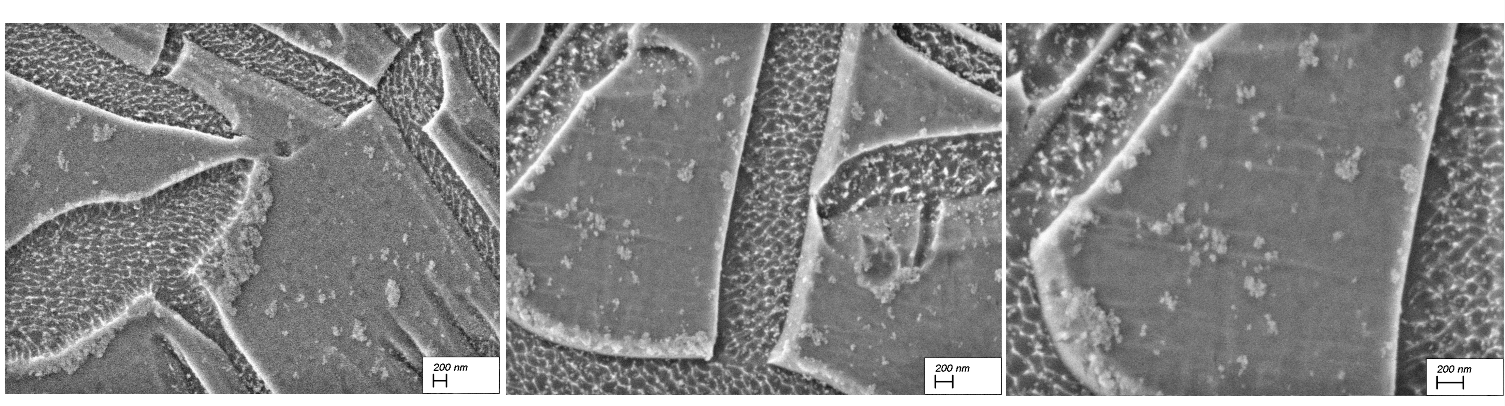
\includegraphics[width=1.0\linewidth]{./Bilder/Abbildung 16.png}
	\caption[Abbildung 16]{983$^\circ$C/1h/AC + 930$^\circ$C/16min/WQ, REM}
	\label{fig:abbildung-16}
\end{figure}

\begin{figure}
	\centering
	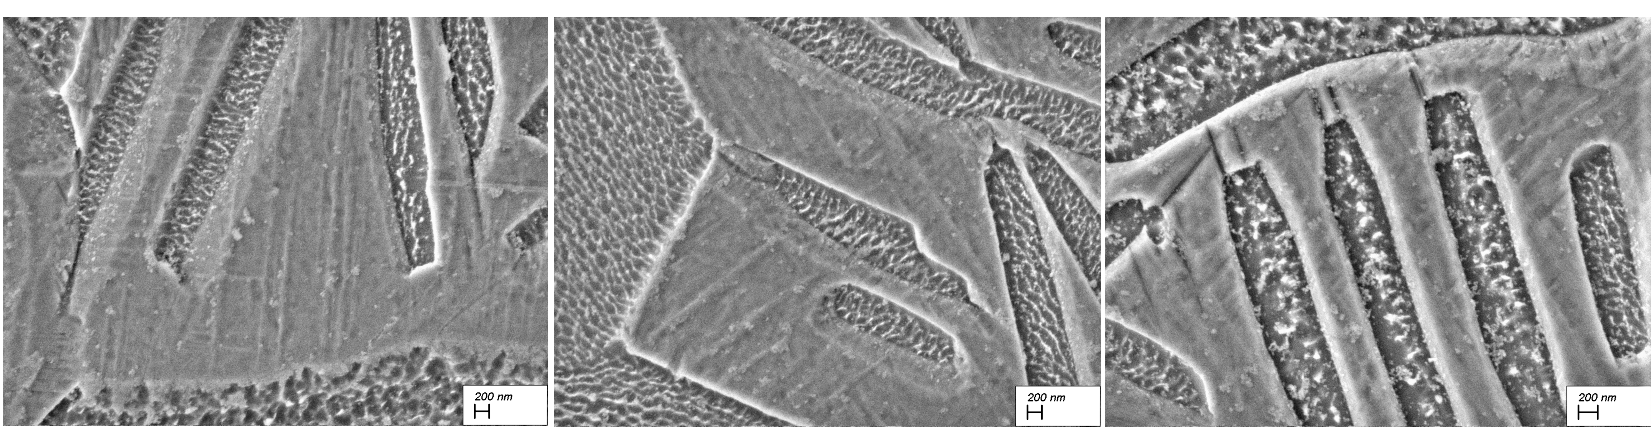
\includegraphics[width=1.0\linewidth]{./Bilder/Abbildung 17.png}
	\caption[Abbildung 17]{983$^\circ$C/1h/AC + 950$^\circ$C/8min/WQ, REM}
	\label{fig:abbildung-17}
\end{figure}

\begin{figure}
	\centering
	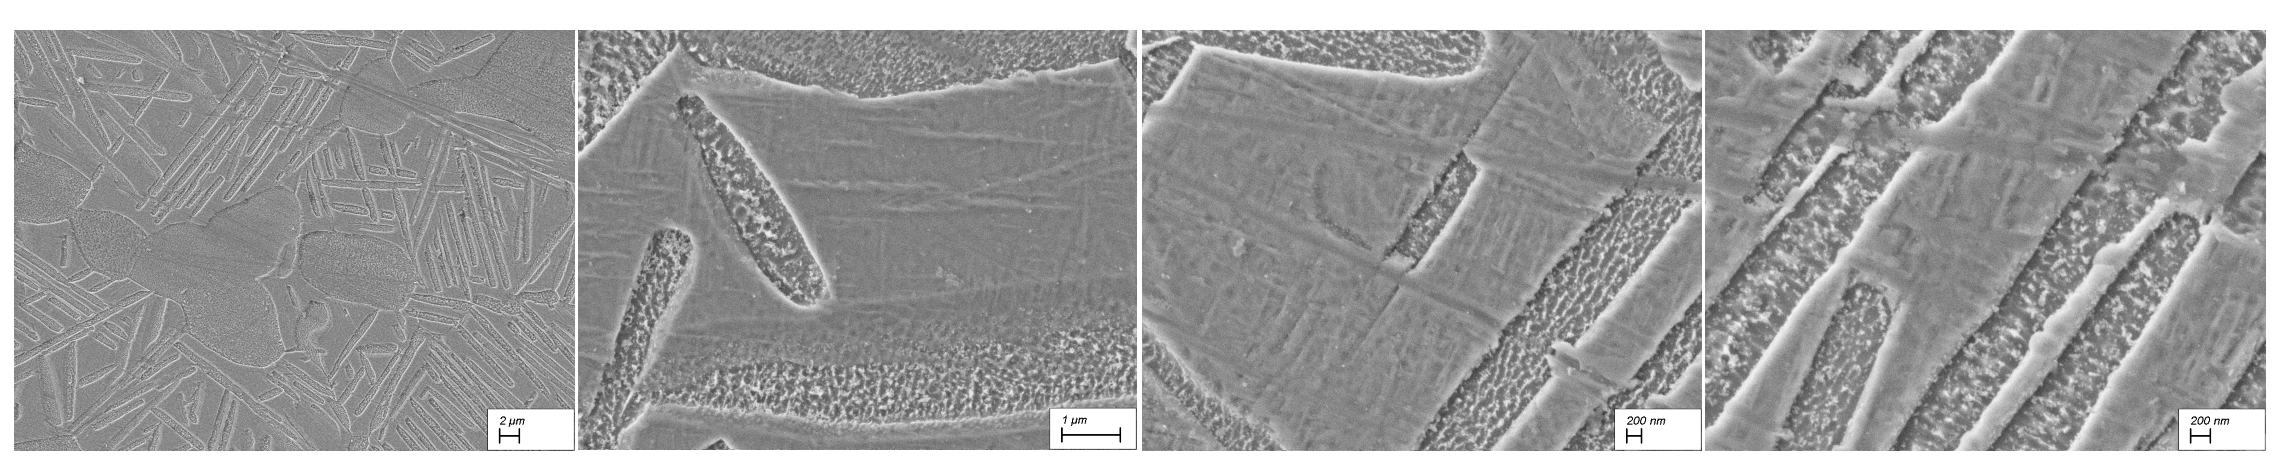
\includegraphics[width=1.0\linewidth]{./Bilder/Abbildung 18.png}
	\caption[Abbildung 18]{983$^\circ$C/1h/AC + 950$^\circ$C/16min/WQ, REM}
	\label{fig:abbildung-18}
\end{figure}

Die Analyse hat gezeigt, dass auch bei der Probe, die bei 930$^\circ$C für 16 Minuten geglüht wurde, ebenfalls nur im Randbereich an vereinzelten Stellen in der $\beta$-Phase leichte martensitische Strukturen erkennbar waren.
Bei den Proben, die bei einer Temperatur von 950$^\circ$C geglüht wurden, sind über der ganzen Probenfläche ausgeprägte martensitische Strukturen zu erkennen. In den Proben mit tieferer Temperatur haben sich lediglich vereinzelt martensitische Strukturen in Bereichen großflächiger $\beta$-Phase im Randbereich gebildet. Bei den Proben, die bei höherer Temperatur geglüht wurden, haben sich auch in den dünneren Flächen der $\beta$-Phase, die zwischen den $\alpha$-Lamellen liegen, ausgeprägte Martensitstrukturen gebildet.


\section{Diskussion der Ergebnisse (ZB)}

Bei  den bei 930  geglühten Proben sind Martensitische Strukturen nur  am Rand und lokal festzustellen. Das zeigt, dass die 8 minütige Anlasszeit nicht ausreichend für die Durchwärmung der Proben war. (960 Proben im vergleich zu den anderen in ergebnisse ? )
(Alpha p studie erklären) - Tabelle 5.1 - 
Außerdem ist die Martensititsche Umwandlung bei der Temperatur  nur an vereinzelten  Stellen zu finden. Deshalb ist die härte dieser Probenreihe nach dem 2-ten Schritt nicht gestiegen(Tabelle 5.2--5.3). Auch bei der Erwärmung für 16 min war kein signifikanter Härteanstieg feststellbar. Das erklärt, dass die Umwandlungskinetik von Alpha zu Beta bei 930$^\circ$C zu niedrig ist, um beta Lamellen  innerhalb von 8--16 min ausreichend  wachsen zu lassen. Diese begrenzte Transformation Alpha Beta bzw. Bildung von instabilen Beta Gebiete führte  beim Abschrecken zu vereinzelten martensitischen Strukturen.
Bei den Proben, die bei 950$^\circ$C für 8 und 16 min geglüht wurden, sind über der ganzen Probenfläche Martensitische Strukturen festzustellen (Verweis auf Bilder). Durch diese Verfeinerung der Gefügestruktur ist die Härte von ca. 340 HV auf 370 HV gestiegen (Tabelle 5.2--5.4). 

